%%%%%%%%%%%%%%%%%%%%%%%%%
\section{Use Cases} \label{useCases}
%%%%%%%%%%%%%%%%%%%%%%%%%
In this chapter some of the possible actions that can be performed into \applicationName\ are presented. The aim of this chapter is to provide a practical introduction to \applicationName, through different use cases.
\subsection{Access information}
The first use case presented introduces the available options to access building data.\\
Whenever a building is selected, an InfoBox is shown through a click of the mouse or a tap on the screen of a smartphone. Figure \ref{subfig:infoBox_city} and Figure \ref{subfig:infoBox} shows how these information are given to the user.\\
\begin{figure} [h]
\centering
	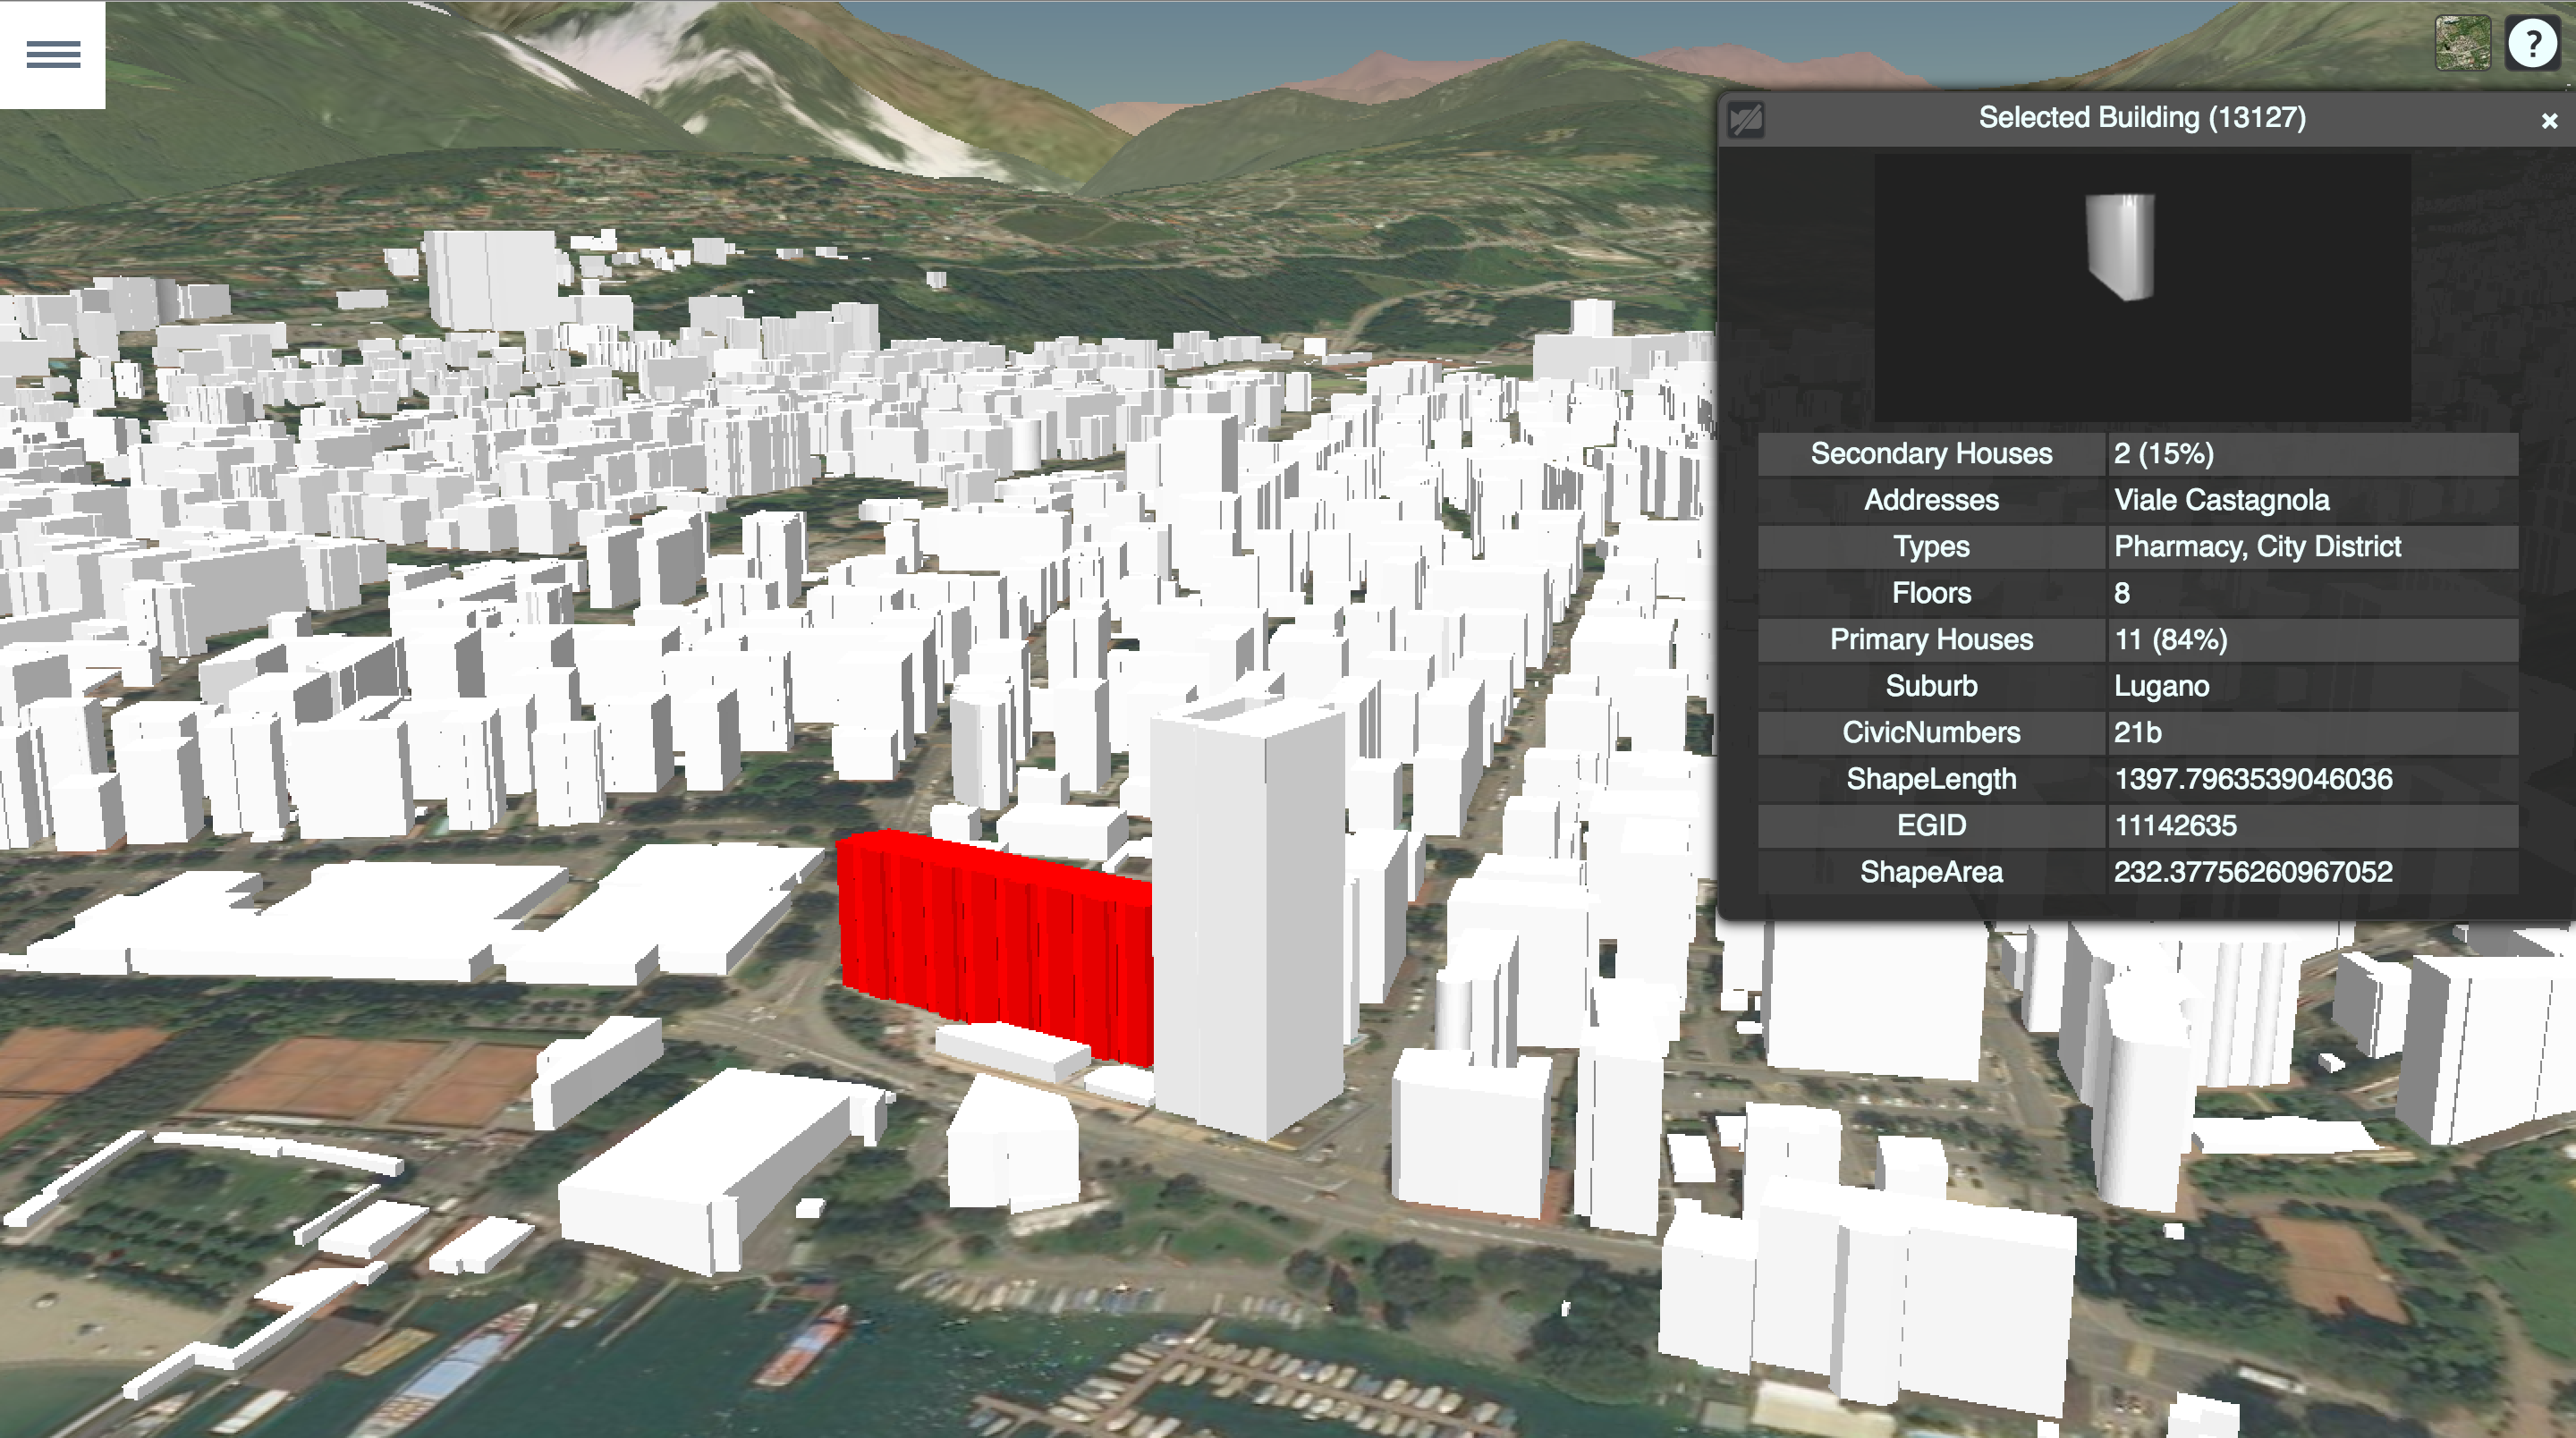
\includegraphics[width=0.8\textwidth]{chapter4/images/infoBox_city}
	\caption{Selecting a building will make the InfoBox appear automatically}
	\label{subfig:infoBox_city}
	\end{figure}
\begin{figure} [h]
	\centering
	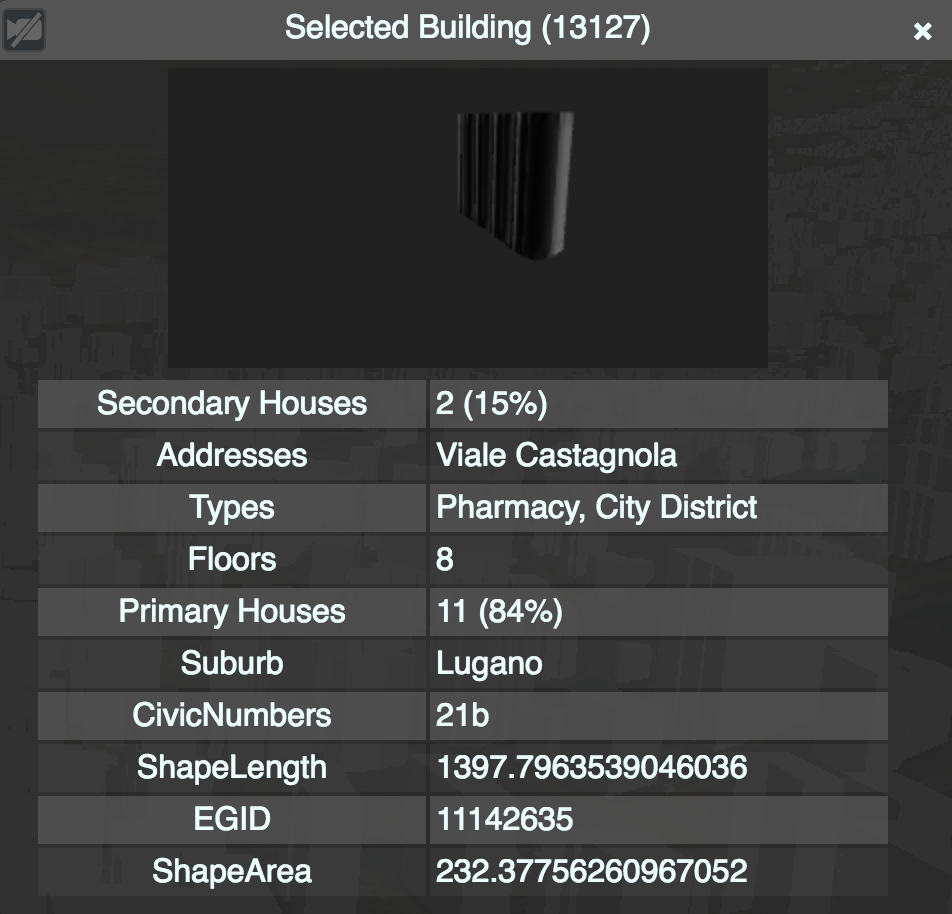
\includegraphics[width=0.5\textwidth]{chapter4/images/infoBox}
	\caption{A detailed look at the InfoBox}
	\label{subfig:infoBox}
\end{figure}
The first field displayed is a 3D representation of the model of the building clicked without its surrounding environment. It is possible to interact with this canvas to freely rotate and zoom the building model.\\
After, a table of useful information about the building follows: the length of this list changes from building to building depending on the available information.\\
The building clicked in the example of Figure \ref{subfig:infoBox} presents all the possible available information that an user can get about a building.\\
The fields of the displayed data are denoted as follows: 
\begin{itemize}
\item {\bf Types} provides the list of groups in which the building is present. Groups are defined by the OpenStreetMap APIs and are used to represent the usage of the buildings which, conceptually, have characteristics in common. Examples of types are: Post Office, Pharmacy, Hospital, University etc \dots.
\item {\bf Floors} is the number of floors of the building
\item {\bf Shape Length \& Shape Area} represent the size of buildings. They are measured in length and area both expressed in meters.
\item {\bf Street Name \& Civic Numbers} are the data concerning the addresses of the street where the building is located. There could be more than one street name and civic numbers in case the building has many of them (e.g., different entrances in the same building that are on different streets). \item {\bf EGID} the unique identifier of the building given by the Swiss REA.
\item {\bf Suburb} represents the suburb in which the building is located.
\item {\bf Primary \& Secondary houses} represents both the number of primary and secondary houses in the selected building and the percentage that each value represents over the total number of houses in that building.
\end{itemize}

\subsection{City Visualization}
The first tab available to the user when the side--bar is opened is the Visualize Tab. It is divided into three main subsections: ``Show on the map'', ``Color city'' and ``Show Suburbs''.\\

The first subsection contains two checkboxes: The first one lets the user show the geolocalization, i.e., the position of the device from which the user is using \applicationName. The second checkbox, if checked, shows the position of webcams located around Lugano. These webcams continuously stream videos of the city. Figure \ref{fig:mapPins} shows the result on the map, when both checkboxes are checked.
\begin{figure} [H]
\centering
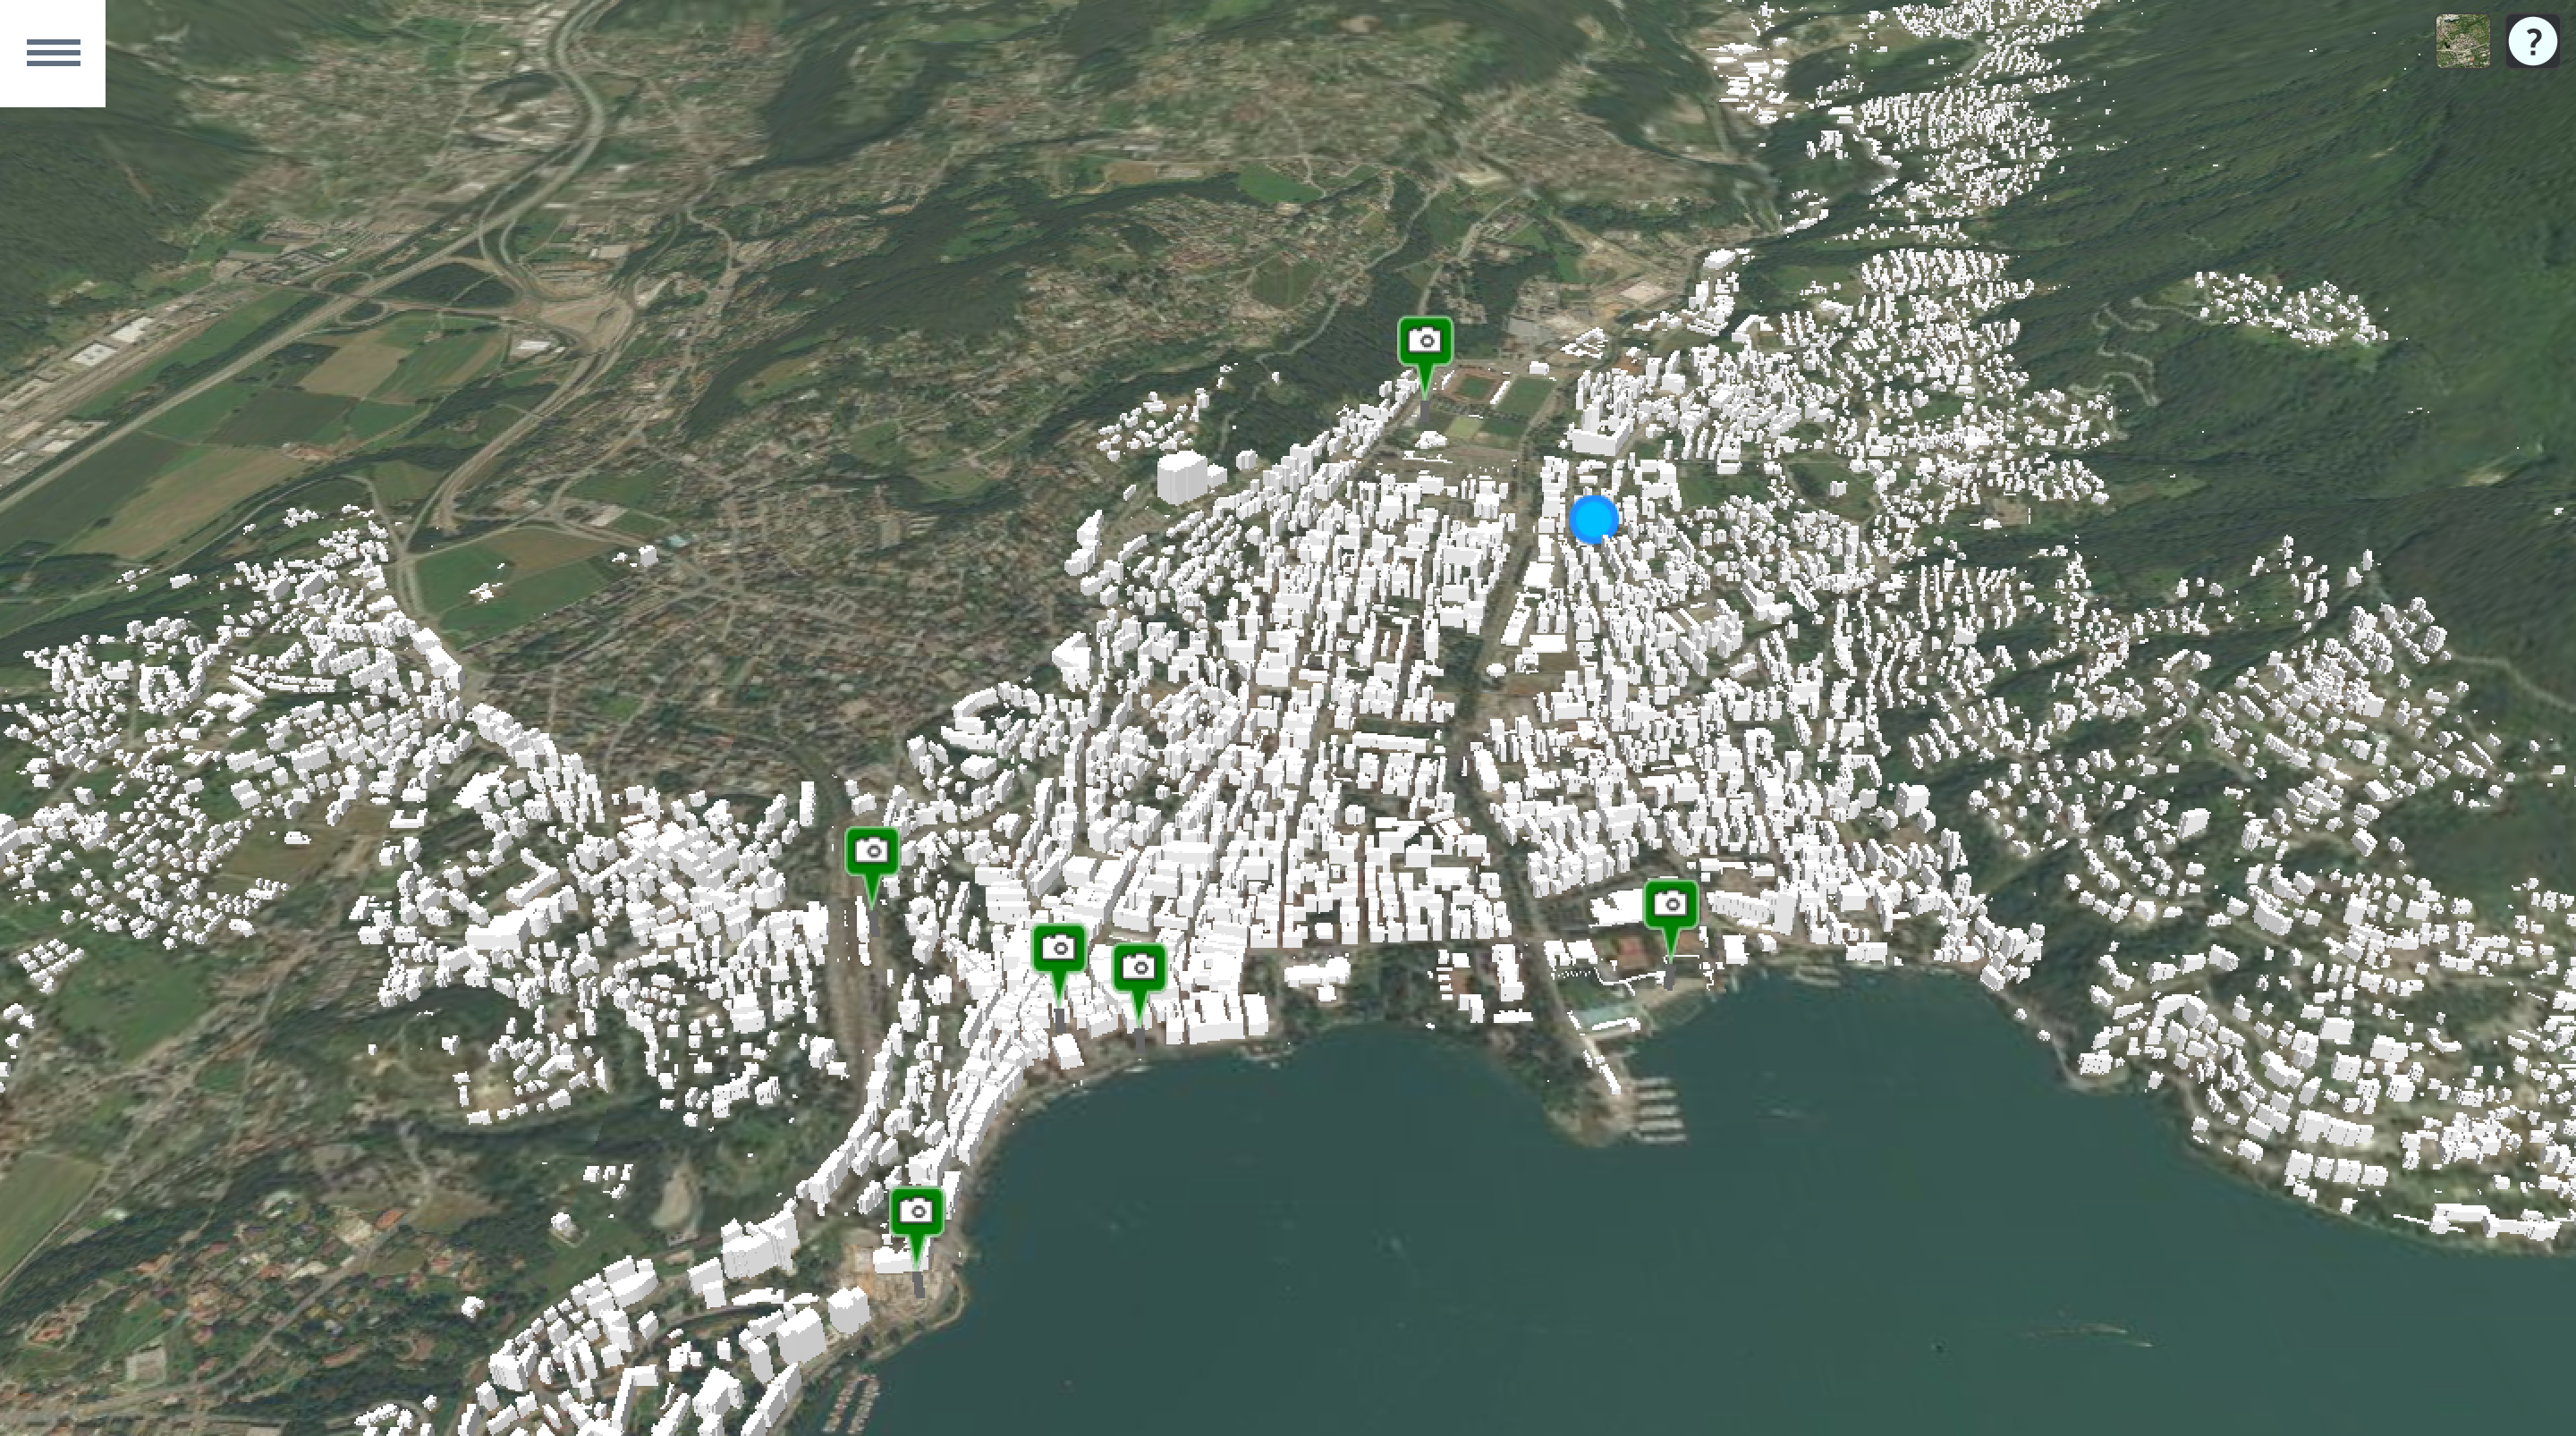
\includegraphics[width=.8\textwidth]{chapter4/images/mapPins}
\caption{When both checkboxes are checked, geolocalization and webCams positions are shown on the map}
\label{fig:mapPins}
\end{figure}
To help the user to exactly locate the position of these pins in the 3D visualization whenever it is more zoomed, a ``stick'' is created starting from the ground and ending at the bottom of the pin, as shown in Figure \ref{fig:3dPins}.\\

\begin{figure} [H]
\centering
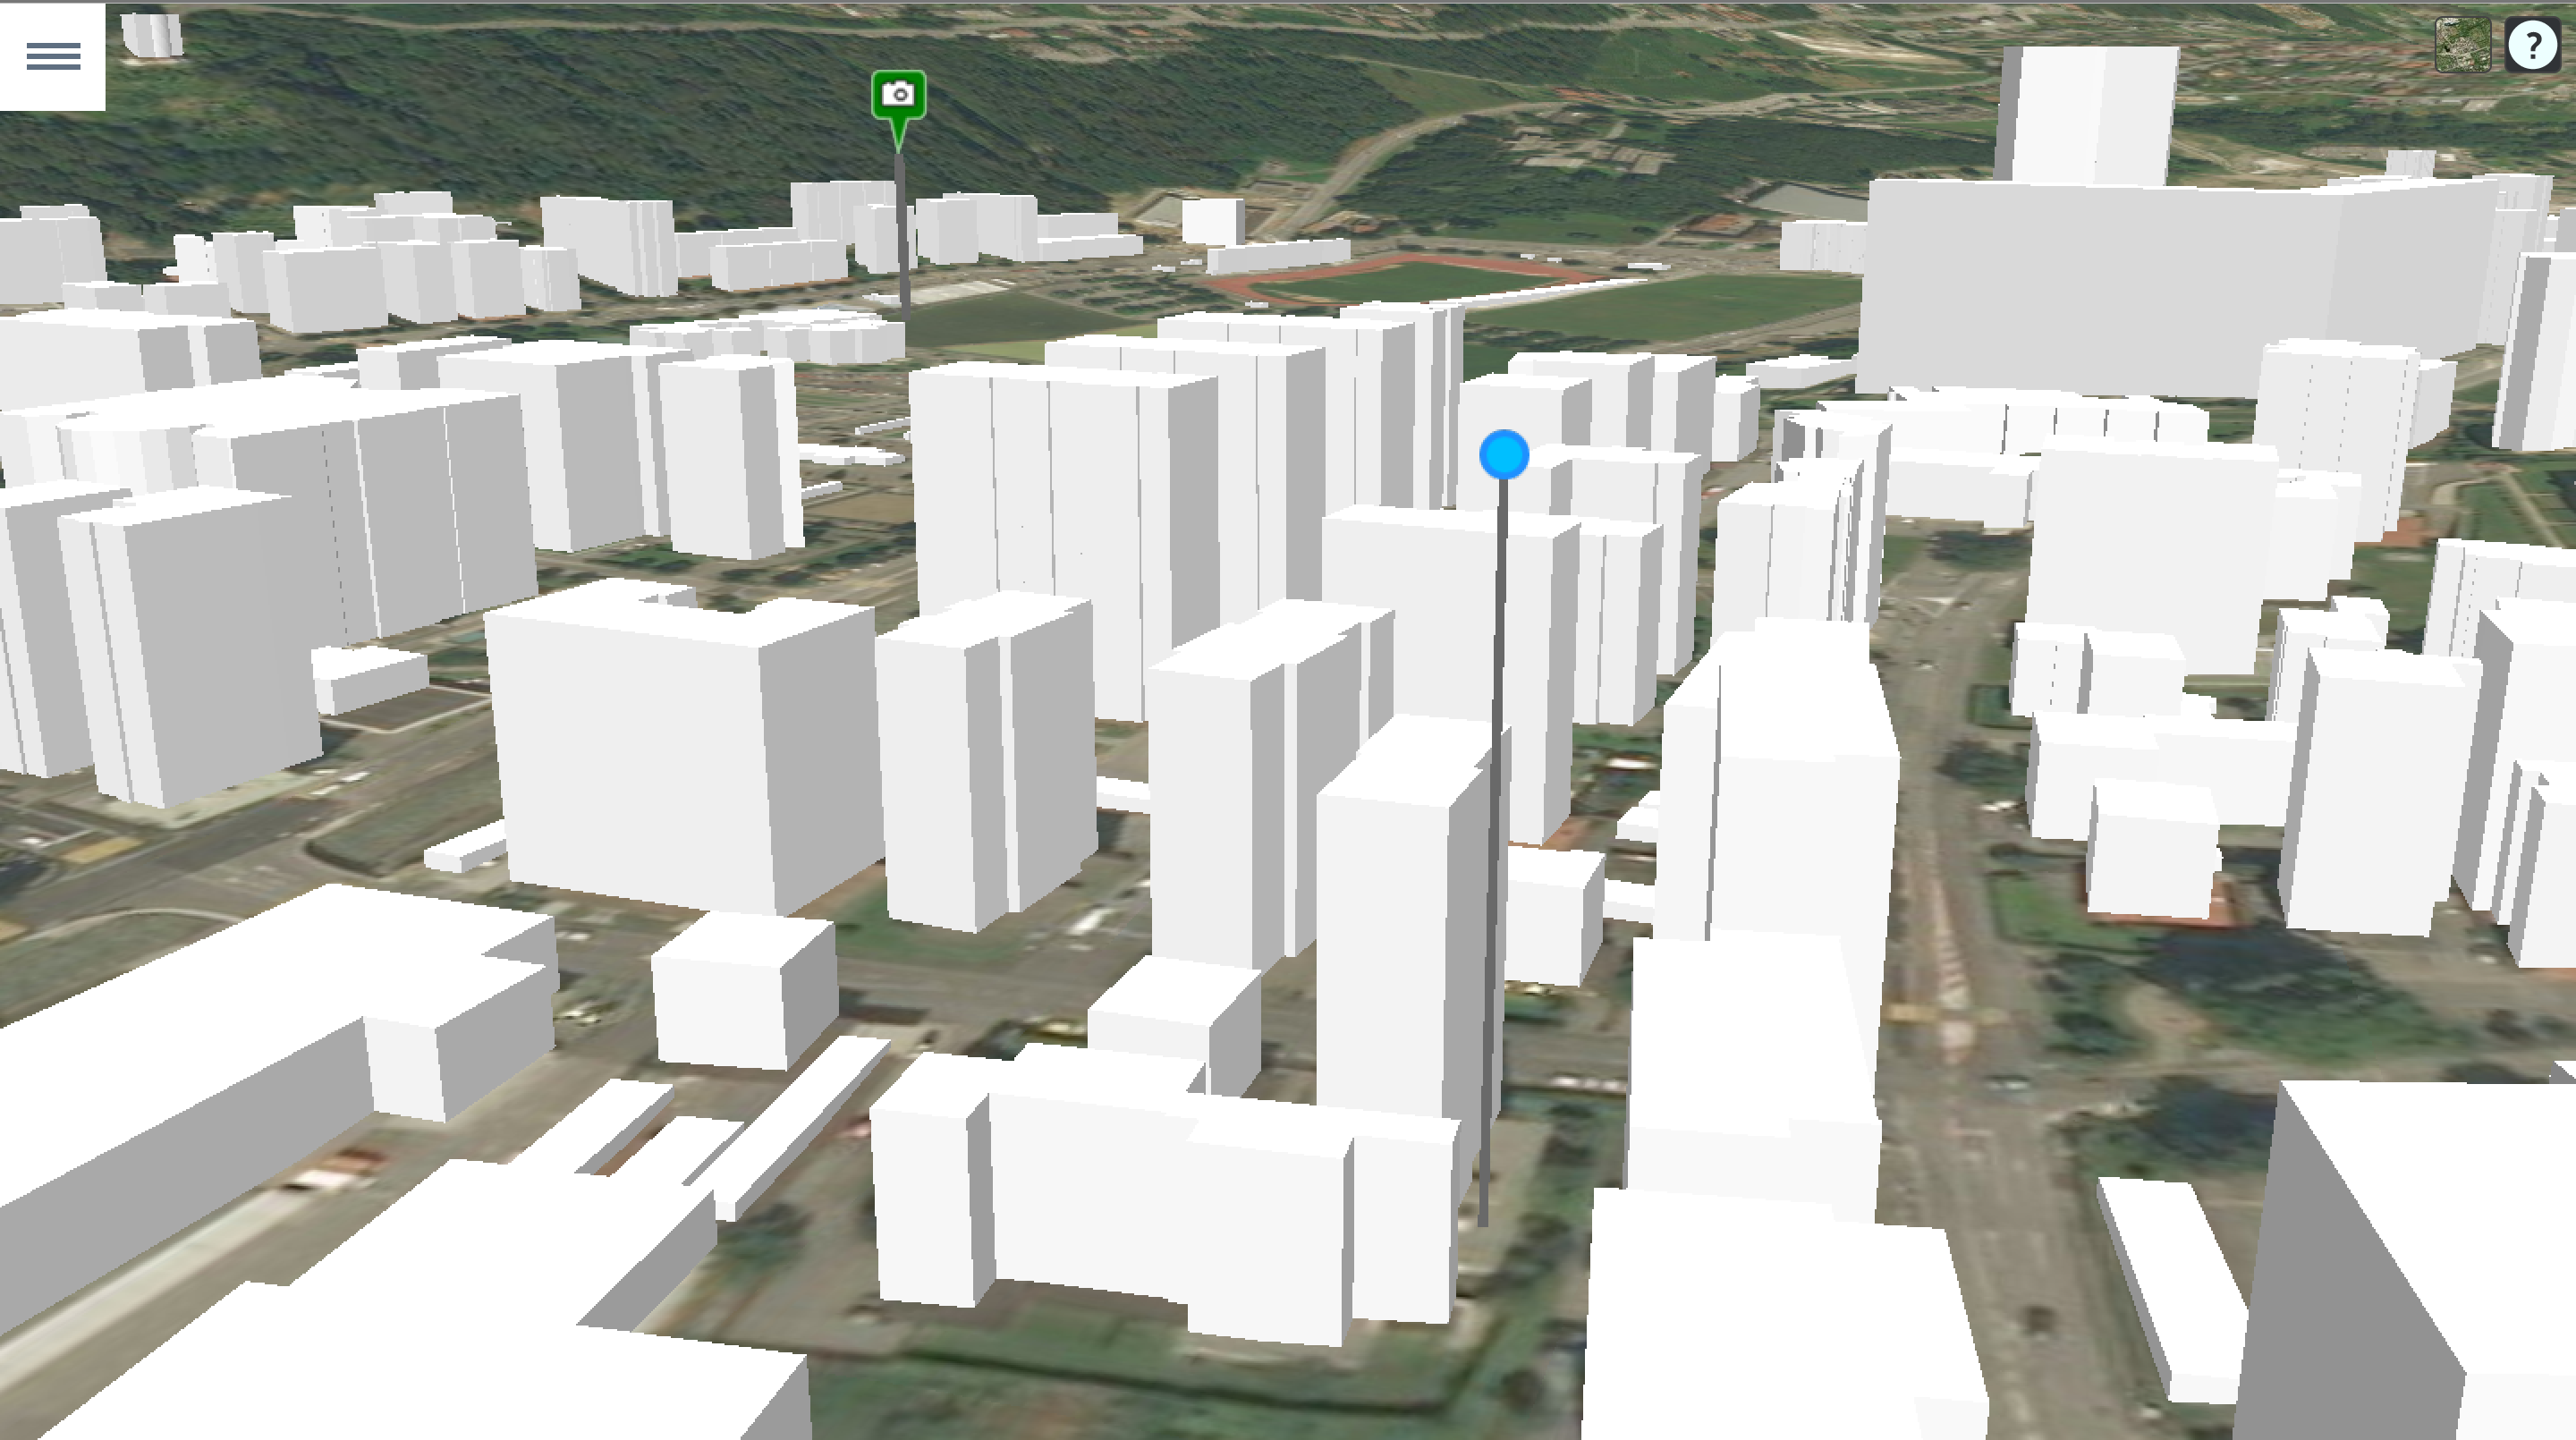
\includegraphics[width=.8\textwidth]{chapter4/images/3dPins}
\caption{The ``Stick'' that connects the ground to the pins}
\label{fig:3dPins}
\end{figure}
In the second subsection three radio buttons can be found: The first one is used to reset the color of the entire city to the default color. The second colors the buildings in the city based on their height (Figure \ref{fig:application_byHeight}). The third one is used to color the entire city based on its suburbs and so every suburb has a different color (Figure \ref{fig:application_showSuburb}).\\

\begin{figure} [H]
\centering
\includegraphics[width=.8\textwidth]{chapter4/images/application_bySuburb}
\caption{A Visualization of the city of Lugano where every suburb is colored differently}
\label{fig:application_bySuburb}
\end{figure}
\begin{figure} [H]
\centering
\includegraphics[width=.8\textwidth]{chapter4/images/application_byHeight}
\caption{A Visualization of the city of Lugano where every building is colored based on its height}
\label{fig:application_byHeight}
\end{figure}
The third and last subsection contains the list of checkboxes representing all the suburbs in the city and their respective colors. By default, all checkboxes are checked: unchecking them will result in hiding the desired suburb as shown in Figure \ref{fig:application_showSuburb}.
\begin{figure} [H]
\centering
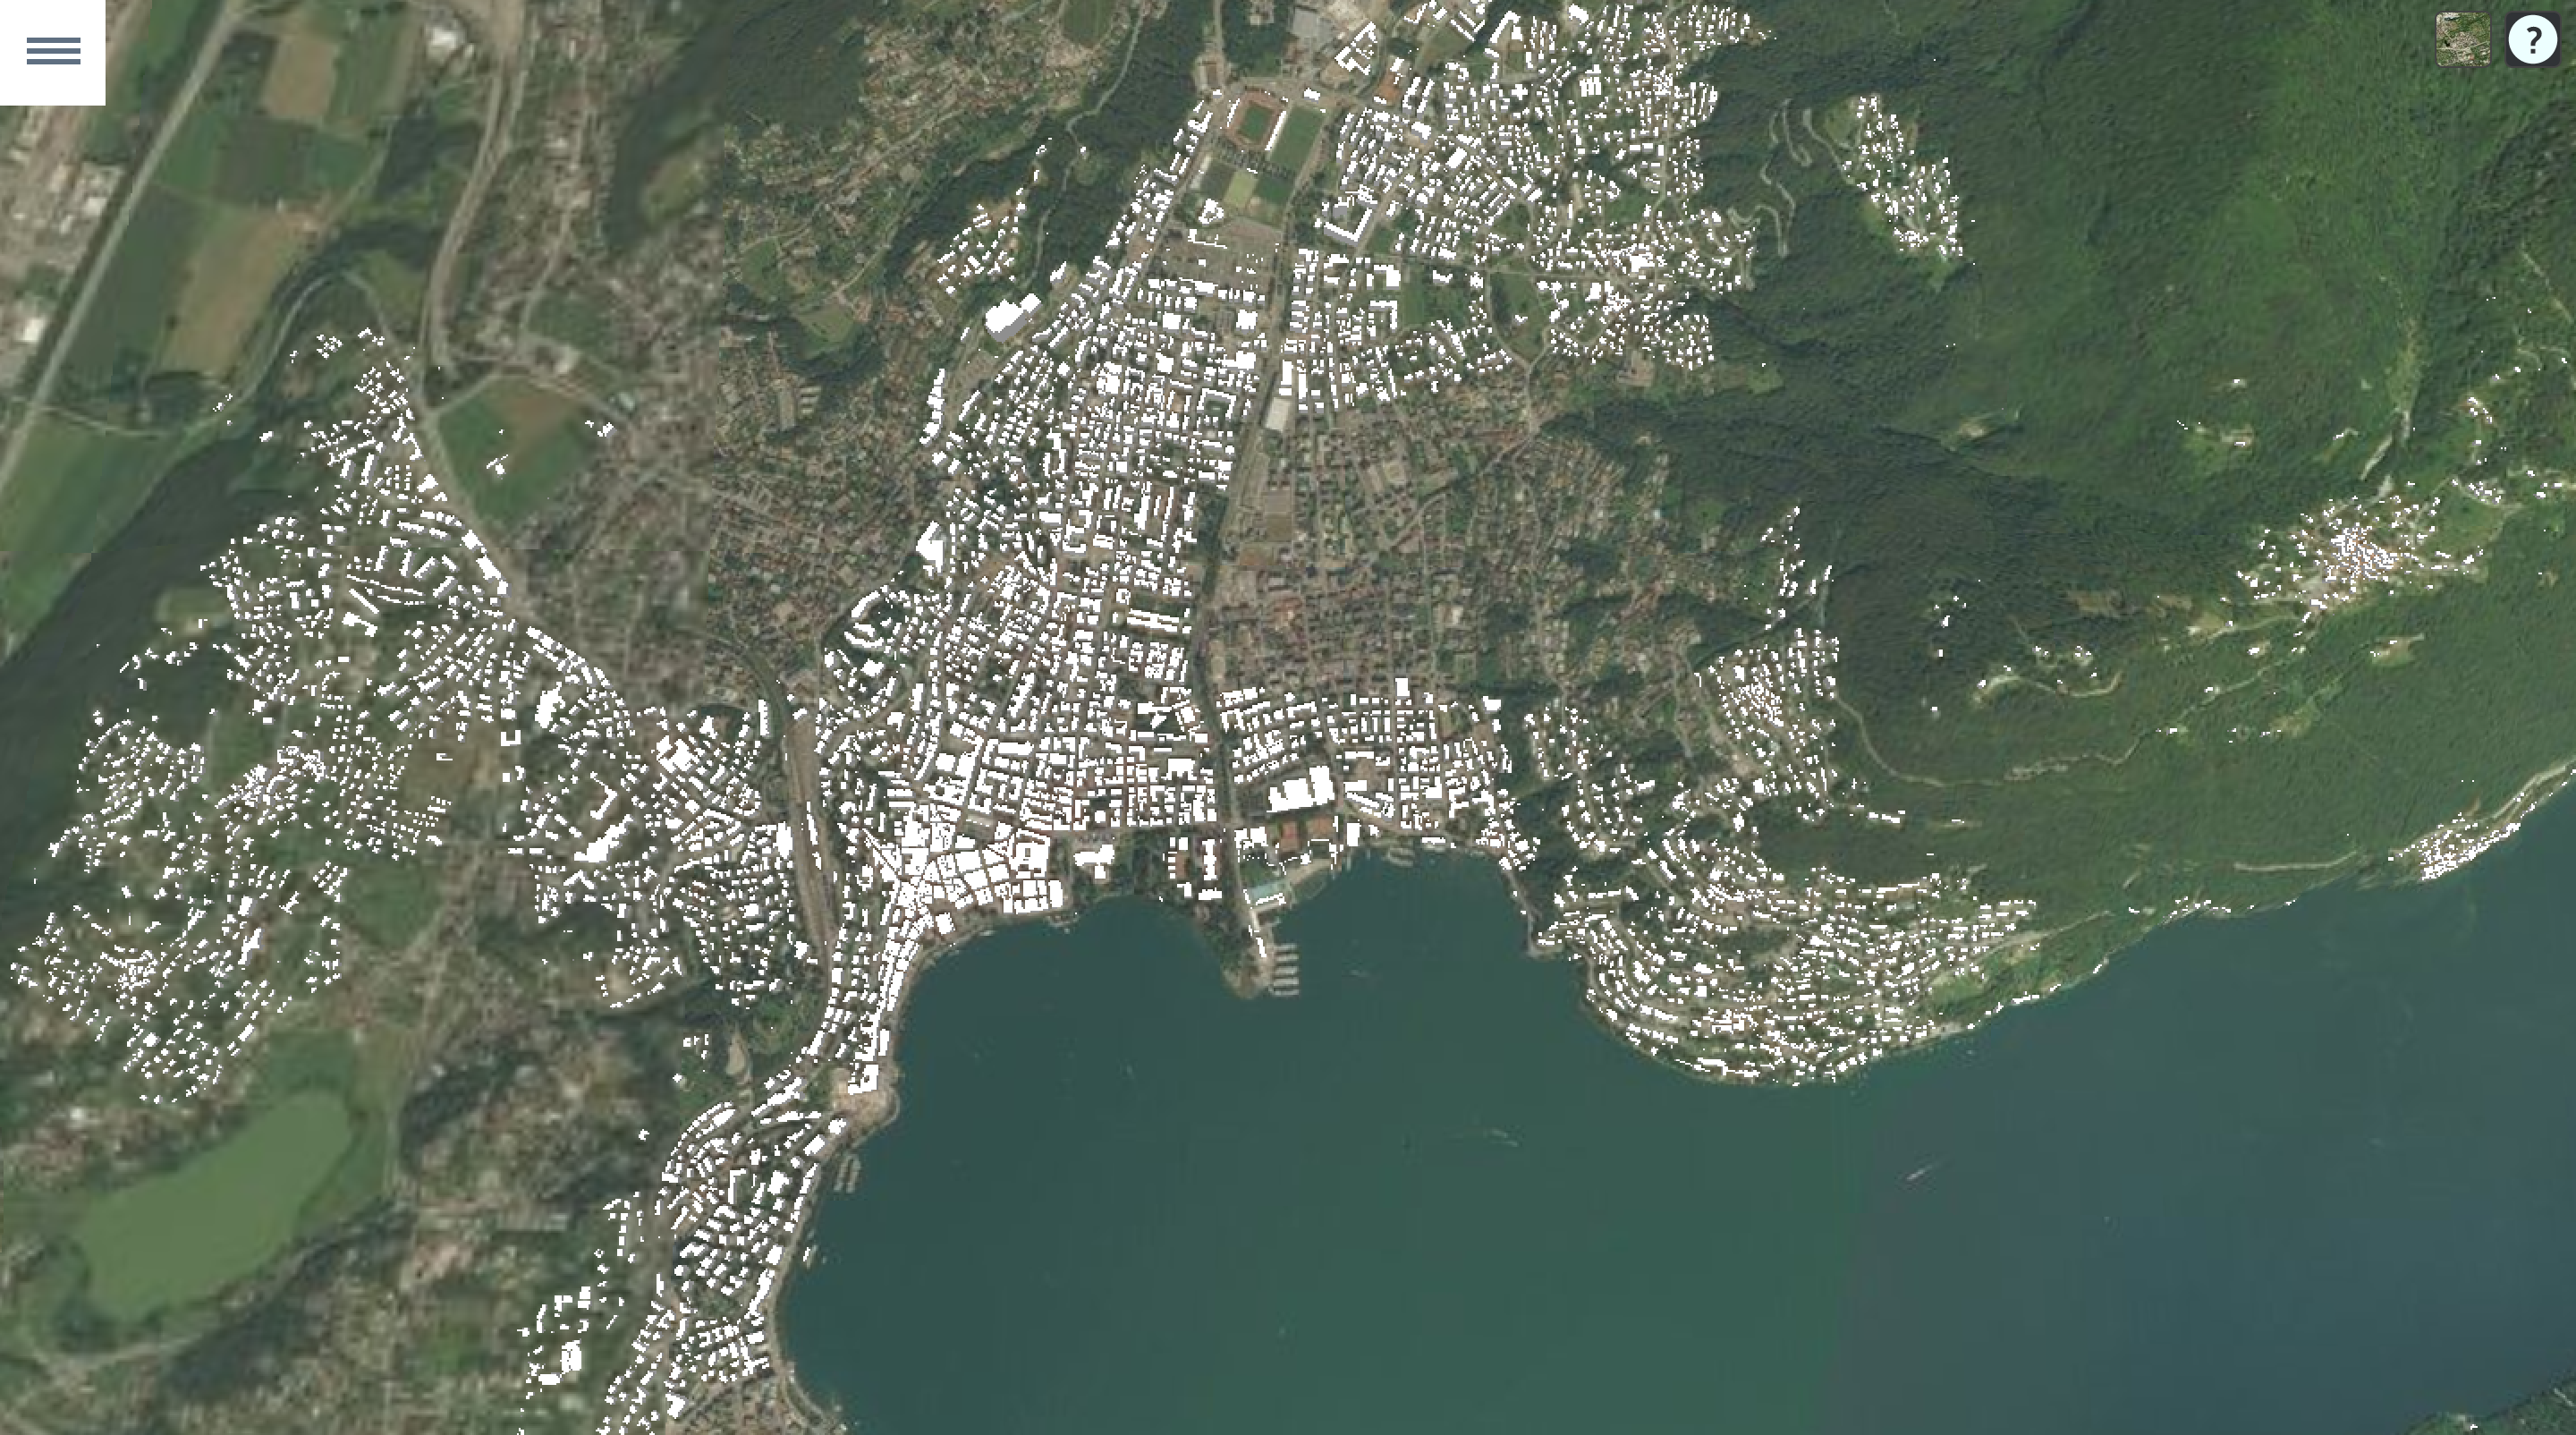
\includegraphics[width=.8\textwidth]{chapter4/images/application_showSuburb}
\caption{A Visualization of the city of Lugano where the suburb Viganello is hidden}
\label{fig:application_showSuburb}
\end{figure}

\subsection{The Query System}
\subsubsection{Building Selection}
The following use cases show what actions can be performed using the visual query system. The interactions proposed are accessible through the apposite ``Query City'' selection tab in the provided sidebar.\\
As shown in Figure \ref{fig:query_city_tab}, \applicationName\ allows the user to perform from very simple to more complex queries on the entire city. Some examples are shown in the following images:
\begin{itemize}
	\item Figure \ref{fig:query1} illustrates the result of the query that looks for all the Banks in the city of Lugano.
	\begin{figure} [H]
\centering
\includegraphics[width=.8\textwidth]{chapter4/images/query1}
\caption{Result of the query: ``Get all the banks in Lugano''}
\label{fig:query1}
\end{figure}  
	\item Figure \ref{fig:query2} shows the result of the query that looks for all the buildings with more than 9 floors in the city of Lugano.
	\begin{figure} [H]
\centering
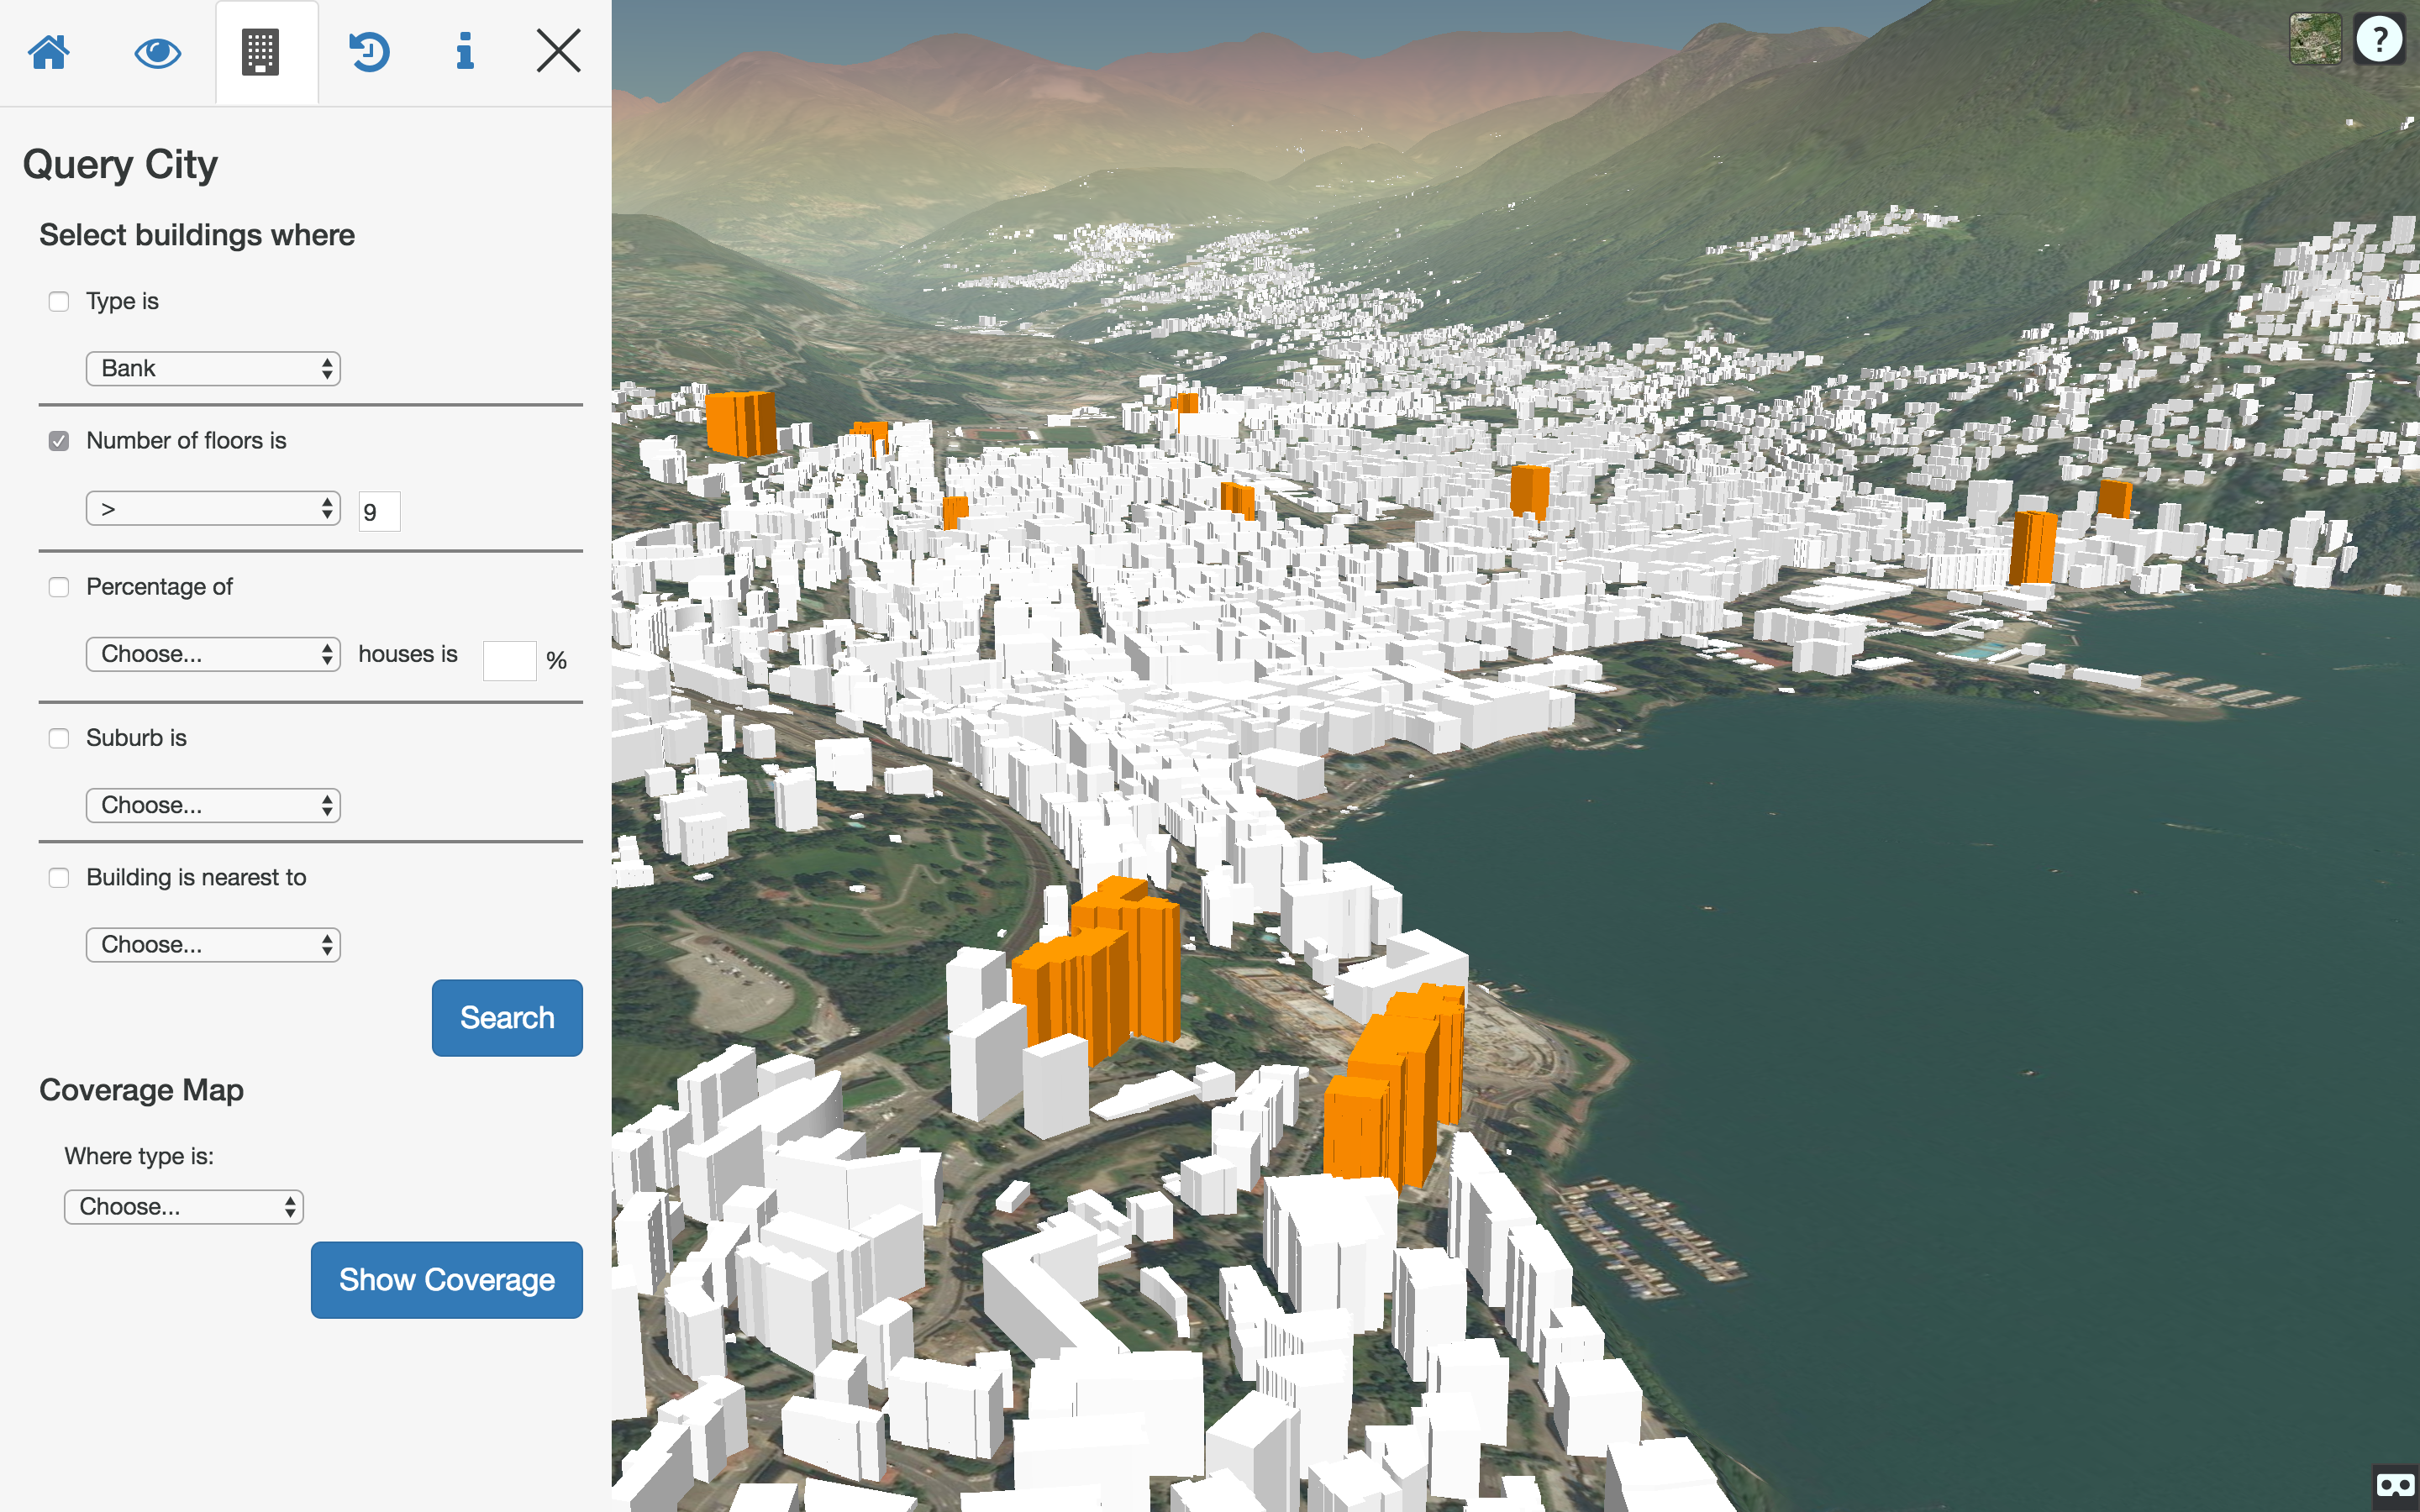
\includegraphics[width=.8\textwidth]{chapter4/images/query2}
\caption{Result of the query: ``Get all the buildings with more than 9 floors in Lugano''}
\label{fig:query2}
\end{figure} 
	\item Figure \ref{fig:query4} corresponds to the result of the query that looks for the building of type Supermarket which is nearest to the selected building.
	\begin{figure} [H]
\centering
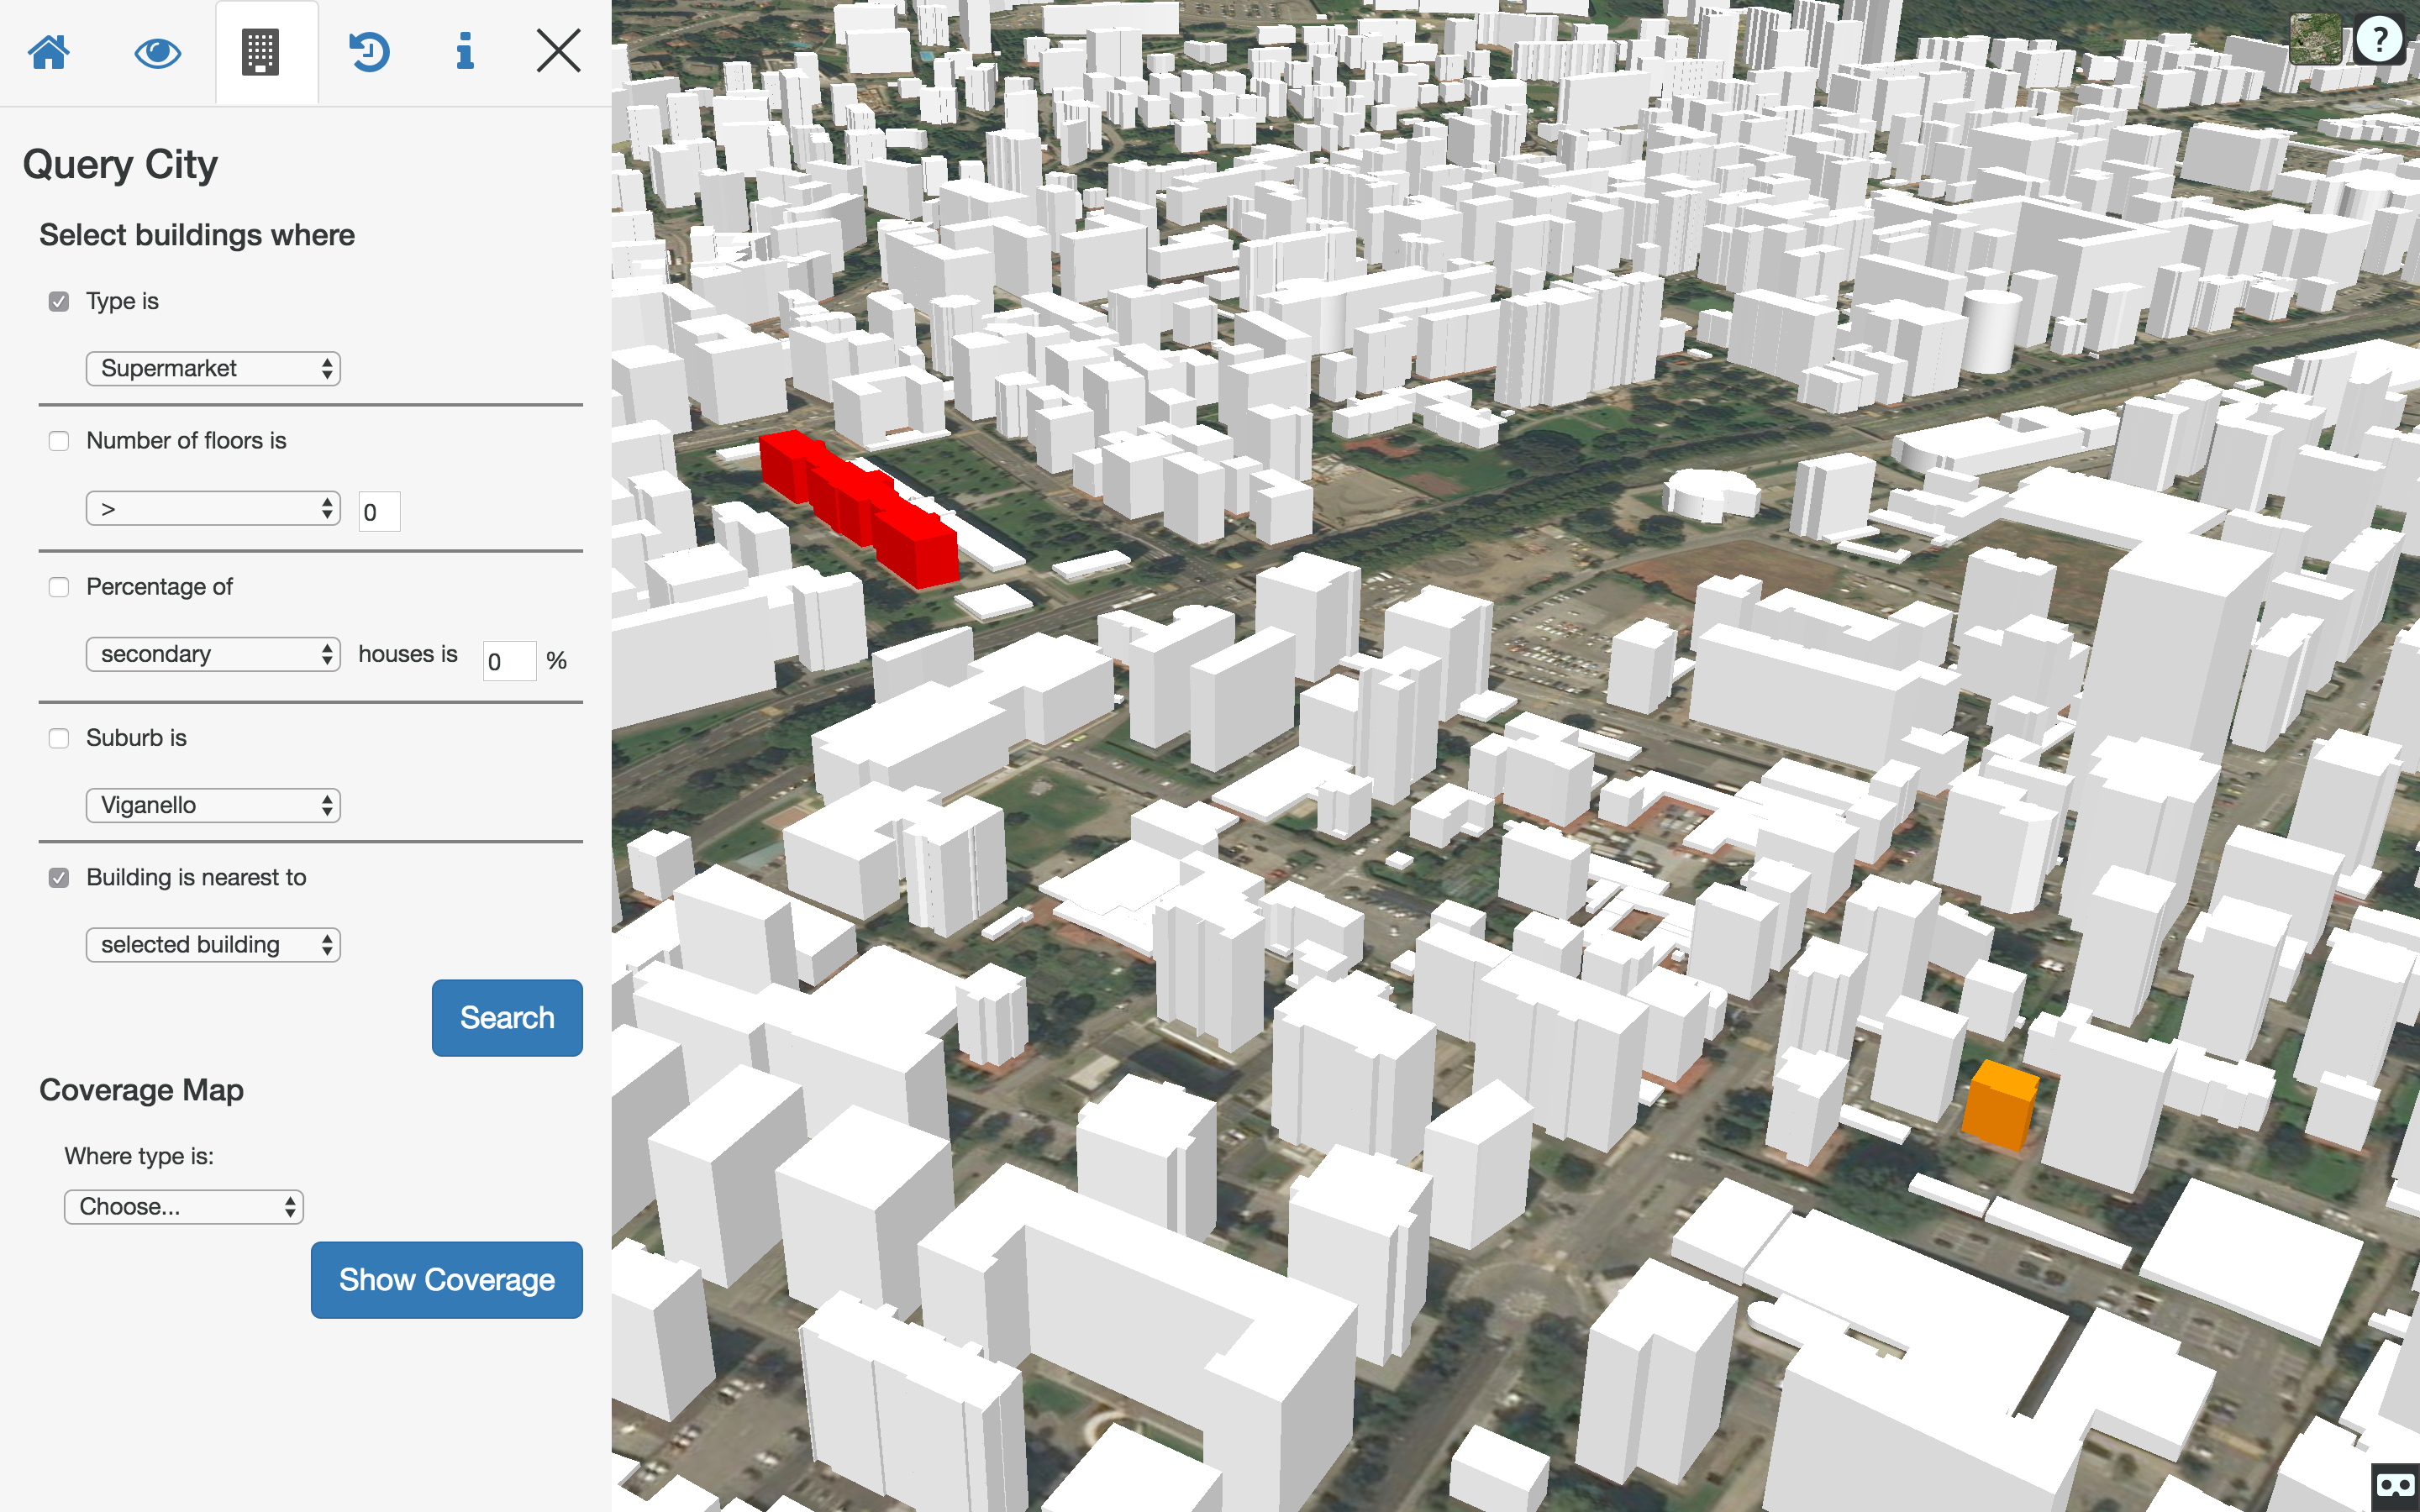
\includegraphics[width=.8\textwidth]{chapter4/images/query4}
\caption{Result of the query: ``Get nearest Supermarket near the selected building''}
\label{fig:query4}
\end{figure} 
	\item  Figure \ref{fig:query5} illustrates the result of the query that looks for all the buildings with less than 10 floors, which have a percentage of primary houses up to the $70\%$, and that are located in the Suburb called Lugano\footnote{Lugano's city centre}.
	\begin{figure} [H]
\centering
\includegraphics[width=.8\textwidth]{chapter4/images/query5}
\caption{Result of the query: ``Get all the buildings with less than 10 floors and where the percentage of primary houses is up to $70\%$ in the Suburb of Lugano''}
\label{fig:query5}
\end{figure} 
\end{itemize}


%\begin{figure} [H]
%\centering
%\includegraphics[width=.8\textwidth]{chapter4/images/query3}
%\caption{Result of the query: ``Get all the hospitals in Viganello (Suburb of Lugano)''}
%\label{fig:query3}
%\end{figure} 



\subsubsection{City Gradient Map}
\applicationName\ also allows visualizing the coverage (i.e., distance of every building from a hotspot) of a specific type--building with respect to the entire city. The coverage is represented by coloring the buildings with a gradient which depends on their distance from a hotspot.\\

In particular, whenever a user does a coverage query, the hotspot or hotspots (in the case of multiple buildings of the same type) will be colored in red. The other buildings will be colored using an interpolation from ``Lime green'' (i.e., the nearest buildings to the hotspost) to white (i.e., the farthest buildings to the hotspot). 
If a building is inside the coverage area of two hotspots, let us say hotspot$_{1}$ and hotspot$_{2}$, its color in RGB will be computed using interpolation from green to white, then the building will take the color given by the most green value (i.e., the one with the smallest values of red and blue). Figure \ref{fig:queryParticular} shows how \applicationName\ represents the color interpolation of buildings depending on their distance from the selected hotspot (or hotspots).

\begin{figure} [H]
\centering
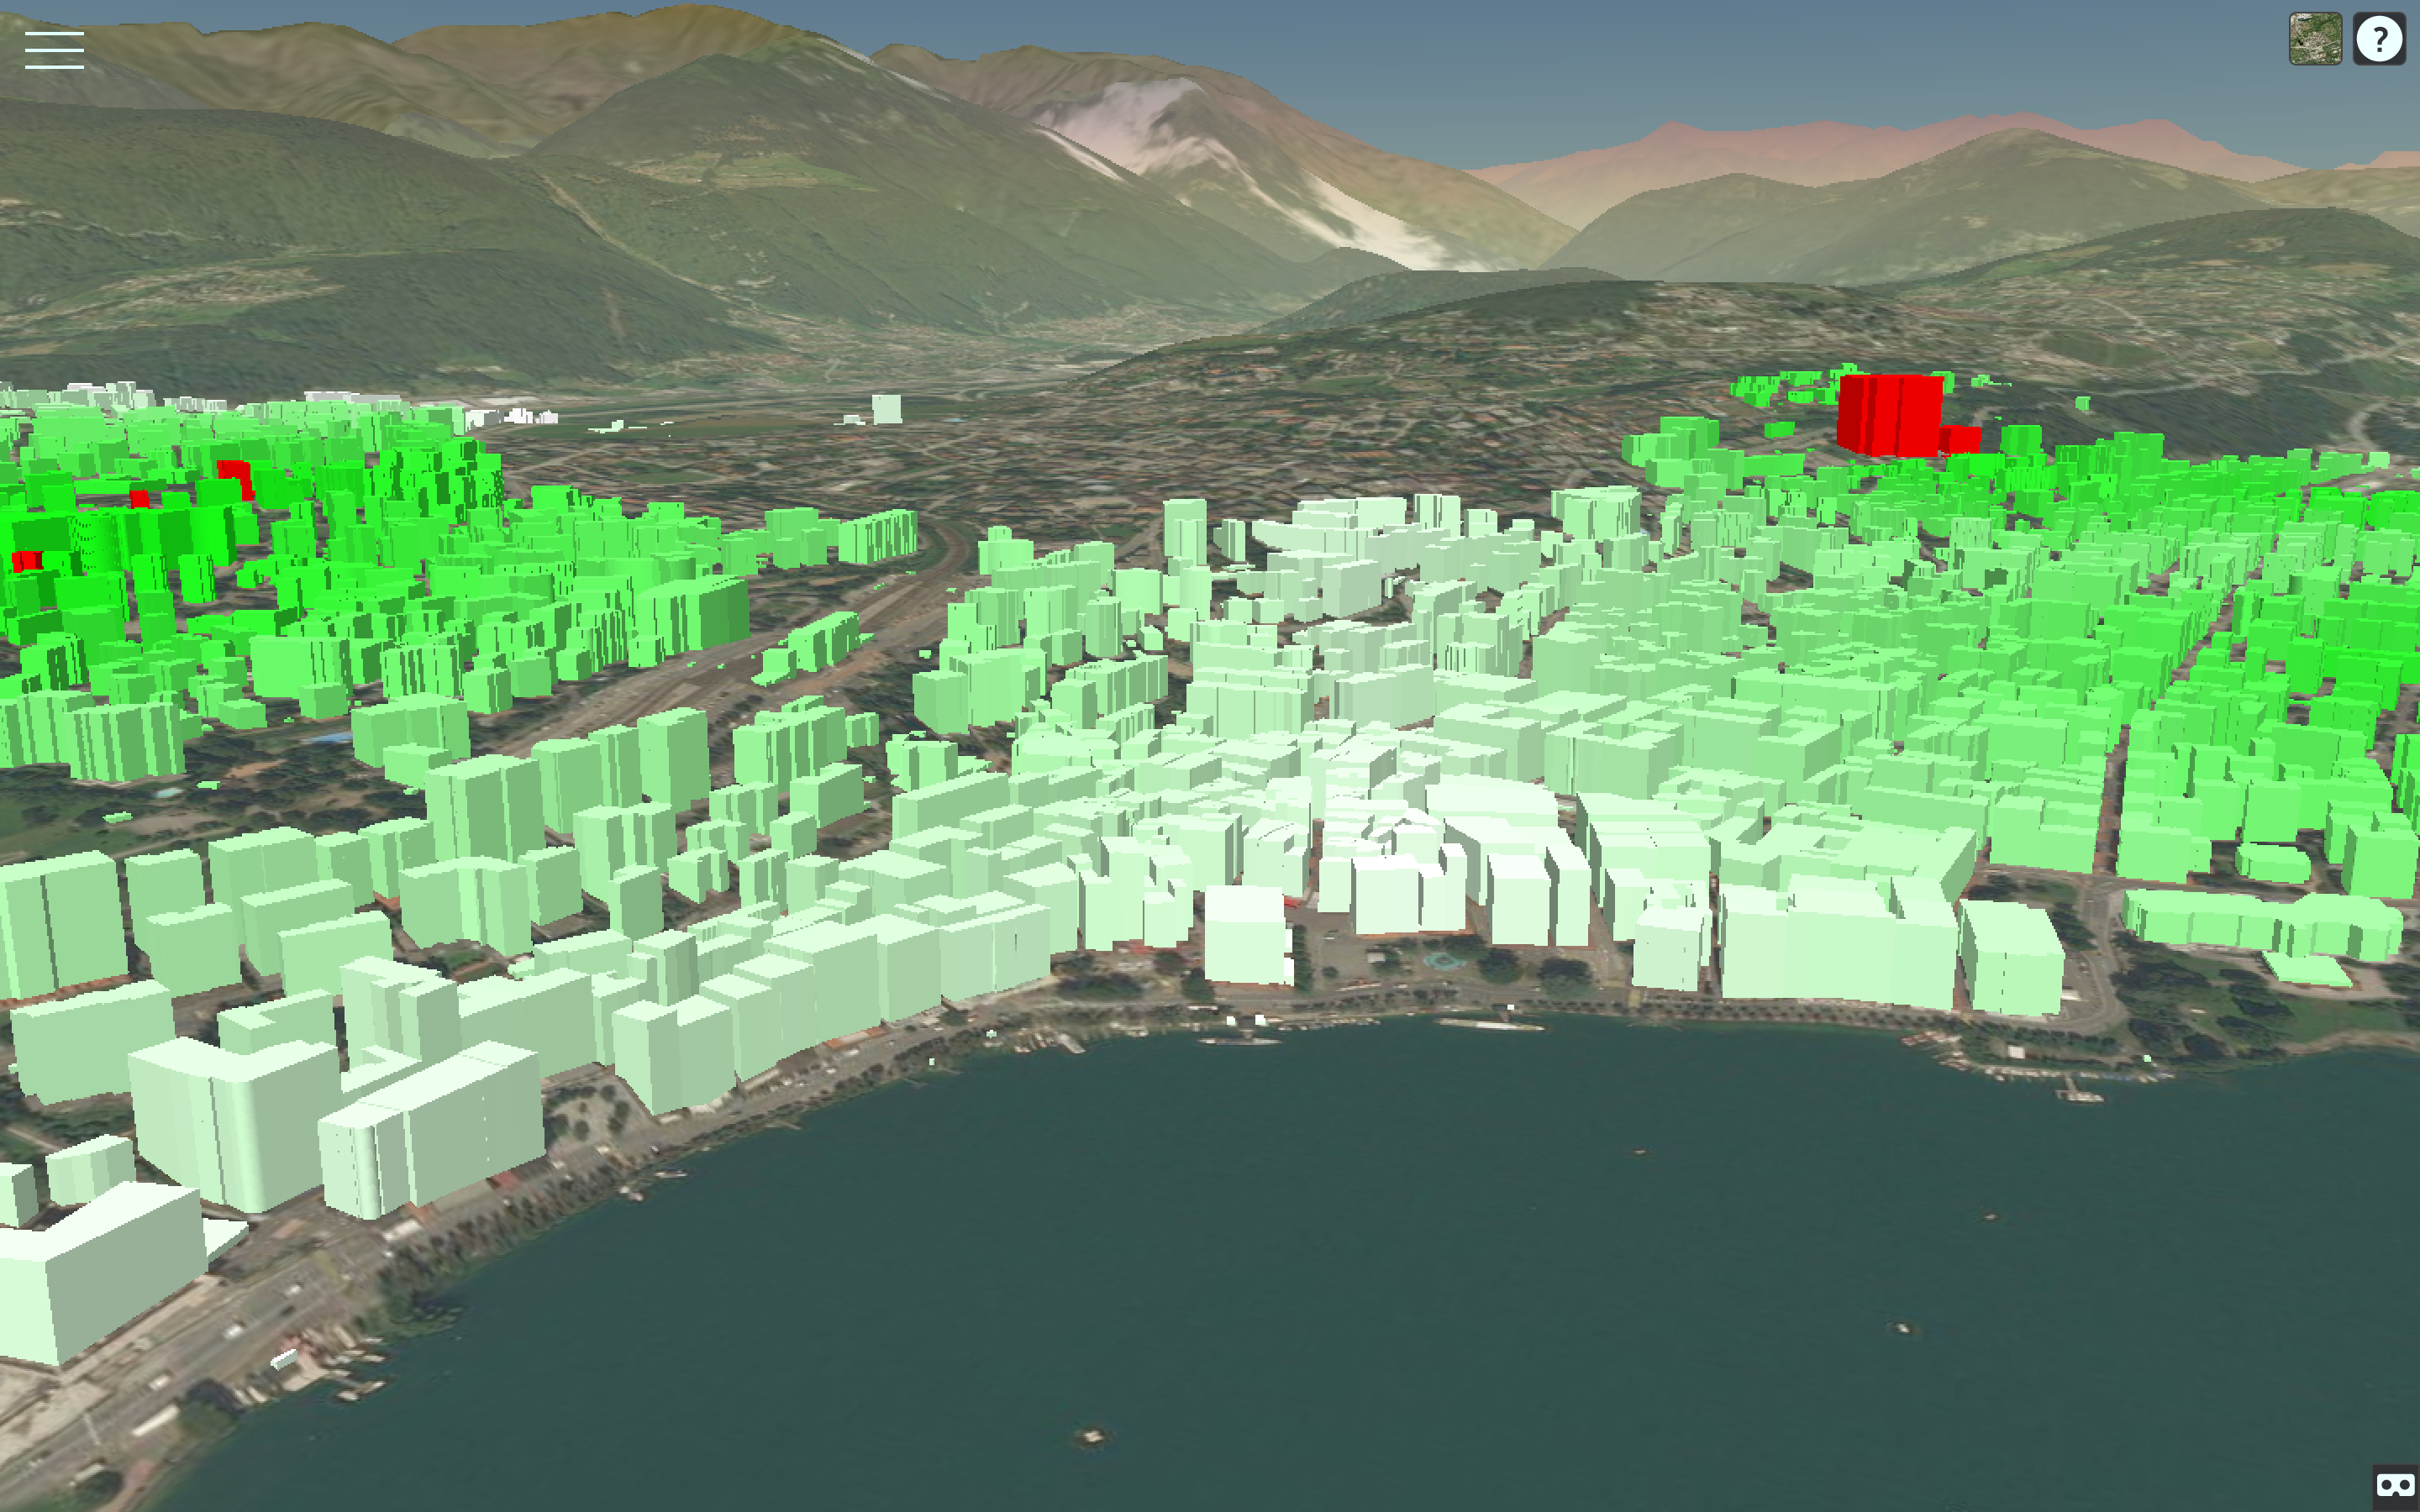
\includegraphics[width=.8\textwidth]{chapter4/images/queryParticular}
\caption{A particular of the result of a query by coverage that shows different shades of green depending on the distance of the building from the hotspot}
\label{fig:queryParticular}
\end{figure} 

Figures \ref{fig:query6} and \ref{fig:query7} show two examples of coverage of a particular hotspot in the city of Lugano. The former represents the coverage of banks, the latter the coverage of hospitals in the city.\\We can determine that the coverage of banks is more distributed in the city of Lugano than the coverage of hospitals. In fact, after the coverage of hospitals is executed, there are suburbs of the city that are completely colored in white since they are very far from this kind of building and, on the other hand, only the suburb called Lugano is highly covered by them.
\begin{figure} [H]
\centering
\includegraphics[width=.8\textwidth]{chapter4/images/query6}
\caption{Coverage map of banks in the city of Lugano}
\label{fig:query6}
\end{figure} 
\begin{figure} [H]
\centering
\includegraphics[width=.8\textwidth]{chapter4/images/query7}
\caption{Coverage map of hospitals in the city of Lugano}
\label{fig:query7}
\end{figure} 
This kind of visualization could be useful for city planning. For example, in the case of the hospitals, the municipal office of the city could decide to build a new hospital in suburbs which are not covered by this type of building since they are too far from them. In this way, \applicationName\ could support decisions that can improve services provided by the city.